\chapter{质量与体积}\label{ch:g6:mass-and-volume}

瓶子里能装多少柠檬水，一箱瓶子有多重？
这是两个不同的问题——一个问占了多大地方，一个问含了多少东西——
而日常说话却随口把它们都叫作同一个字：“大”。科学
则把两者区分开来：体积指物体所占的空间，
质量指物体所含物质的多少。测量质量，你早已
驾轻就熟；今天我们来学习测量体积——哪怕是
一颗形状不规则、尺子都无从量起的小石子。

\section{体积：物体所占的空间}

\begin{definition}[体积]\label{def:g6:mass-and-volume:volume}
物体的\emph{体积}\index{体积}是指它
所占空间的大小。固体、液体和气体都有体积：砖块
占据自己的空间，柠檬水占据瓶子的内部，空气占据其余的部分。
体积的常用单位是
\emph{立方厘米}\index{立方厘米}（\unit{cm^3}）——即棱长为一厘米的
小立方体所占的空间——还有
\emph{升}\index{升}（\unit{L}）。
\end{definition}

\begin{proposition}[立方体中的升]\label{prop:g6:mass-and-volume:litre}
体积的两类单位实际上是同一类：
\[
\qty{1}{L} = \qty{1000}{cm^3},
\qquad
\qty{1}{mL} = \qty{1}{cm^3}.
\]
一升恰好等于棱长为十厘米的正方体
所占的空间：$10 \times 10 \times 10 = 1000$ 个小立方体。
\end{proposition}

\begin{omfigure}
\begin{tikzpicture}[scale=0.85]
  \draw[thick] (0,0) rectangle (3,3);
  \draw[thick] (0,3) -- (0.9,3.75) -- (3.9,3.75) -- (3,3);
  \draw[thick] (3.9,3.75) -- (3.9,0.75) -- (3,0);
  \foreach \i in {1,...,9} {
    \draw[very thin] (0,0.3*\i) -- (3,0.3*\i);
    \draw[very thin] (0.3*\i,0) -- (0.3*\i,3);
    \draw[very thin] (0.3*\i,3) -- (0.3*\i+0.9,3.75);
    \draw[very thin] (3,0.3*\i) -- (3.9,0.3*\i+0.75);
    \draw[very thin] (0.09*\i,3+0.075*\i) -- (3+0.09*\i,3+0.075*\i);
    \draw[very thin] (3+0.09*\i,0.075*\i) -- (3+0.09*\i,3+0.075*\i);
  }
  \draw[thick, fill=omDef, fill opacity=0.6]
    (0,2.7) rectangle (0.3,3);
  \node[right, font=\small] at (4.6,3.0)
    {大立方体：每条棱长 \qty{10}{cm}};
  \node[right, font=\small] at (4.6,2.2)
    {$10 \times 10 \times 10 = 1000$ 个小立方体};
  \node[right, font=\small] at (4.6,1.4)
    {每个小立方体：\qty{1}{cm^3}};
  \node[right, font=\small, omDef] at (4.6,0.6)
    {合计：$\qty{1000}{cm^3} = \qty{1}{L}$};
\end{tikzpicture}

{\small 一升拆开来看：一千个立方厘米的小块，
堆成十乘十乘十的大方块。}
\end{omfigure}

\begin{example}[需要熟记的体积]\label{ex:g6:mass-and-volume:byheart}
一茶匙约能盛\qty{5}{mL}；一只玻璃杯约能盛
\qty{25}{cL}，即四分之一升；一盒牛奶约
\qty{1}{L}；一个浴缸约能盛\qty{150}{L}；一块方糖约占
\qty{3}{cm^3}；一颗骰子约占\qty{4}{cm^3}。这些标准量
能帮助人们判断每次测量结果是否合理。
\end{example}

\section{测量液体}

\begin{method}[读取量筒]\label{met:g6:mass-and-volume:cylinder}
实验室用的量具是\emph{量筒}：细而高，
刻度精细。
\begin{enumerate}
  \item 把量筒放在平整的桌面上——切勿
        手持读数；
  \item 找出刻度值，与读其他任何刻度一样；
  \item 使视线与液面齐平。液面并非
        平的，而是略微弯曲，形成一个
        \emph{弯月面}\index{弯月面}——
        沿玻璃壁略微上爬；
  \item 在弯月面的\emph{底部}处，水平视线读数。
\end{enumerate}
视线过高或过低，弯月面就会骗你读错一两个
刻度——这正是斜视误差最爱披上的外衣。
\end{method}

\begin{omfigure}
\begin{tikzpicture}[scale=0.85]
  \draw[thick] (1.0,0) -- (1.0,4.2) (3.0,0) -- (3.0,4.2);
  \draw[thick] (1.0,0) -- (3.0,0);
  \fill[omDef, opacity=0.2] (1.0,0.05) rectangle (3.0,2.6);
  \draw[omDef, very thick]
    (1.0,2.75) .. controls (1.6,2.55) and (2.4,2.55) .. (3.0,2.75);
  \foreach \y/\l in {0.6/10, 1.4/20, 2.2/30, 3.0/40, 3.8/50} {
    \draw (3.0,\y) -- (3.25,\y);
    \node[right, font=\footnotesize] at (3.3,\y) {\l};
  }
  \draw[-Stealth, omThm, thick] (6.3,2.6) -- (2.2,2.6);
  \node[right, font=\small, omThm] at (6.4,2.6)
    {在弯月面底部读数：\qty{28}{mL}};
  \node[below, font=\small] at (2.0,-0.35)
    {视线与液面齐平，量筒放在桌面上};
\end{tikzpicture}

{\small 弯月面：液体沿玻璃壁略微上爬。正确
的读数位于弯月面底部，视线与液面齐平。}
\end{omfigure}

\begin{omfigure}
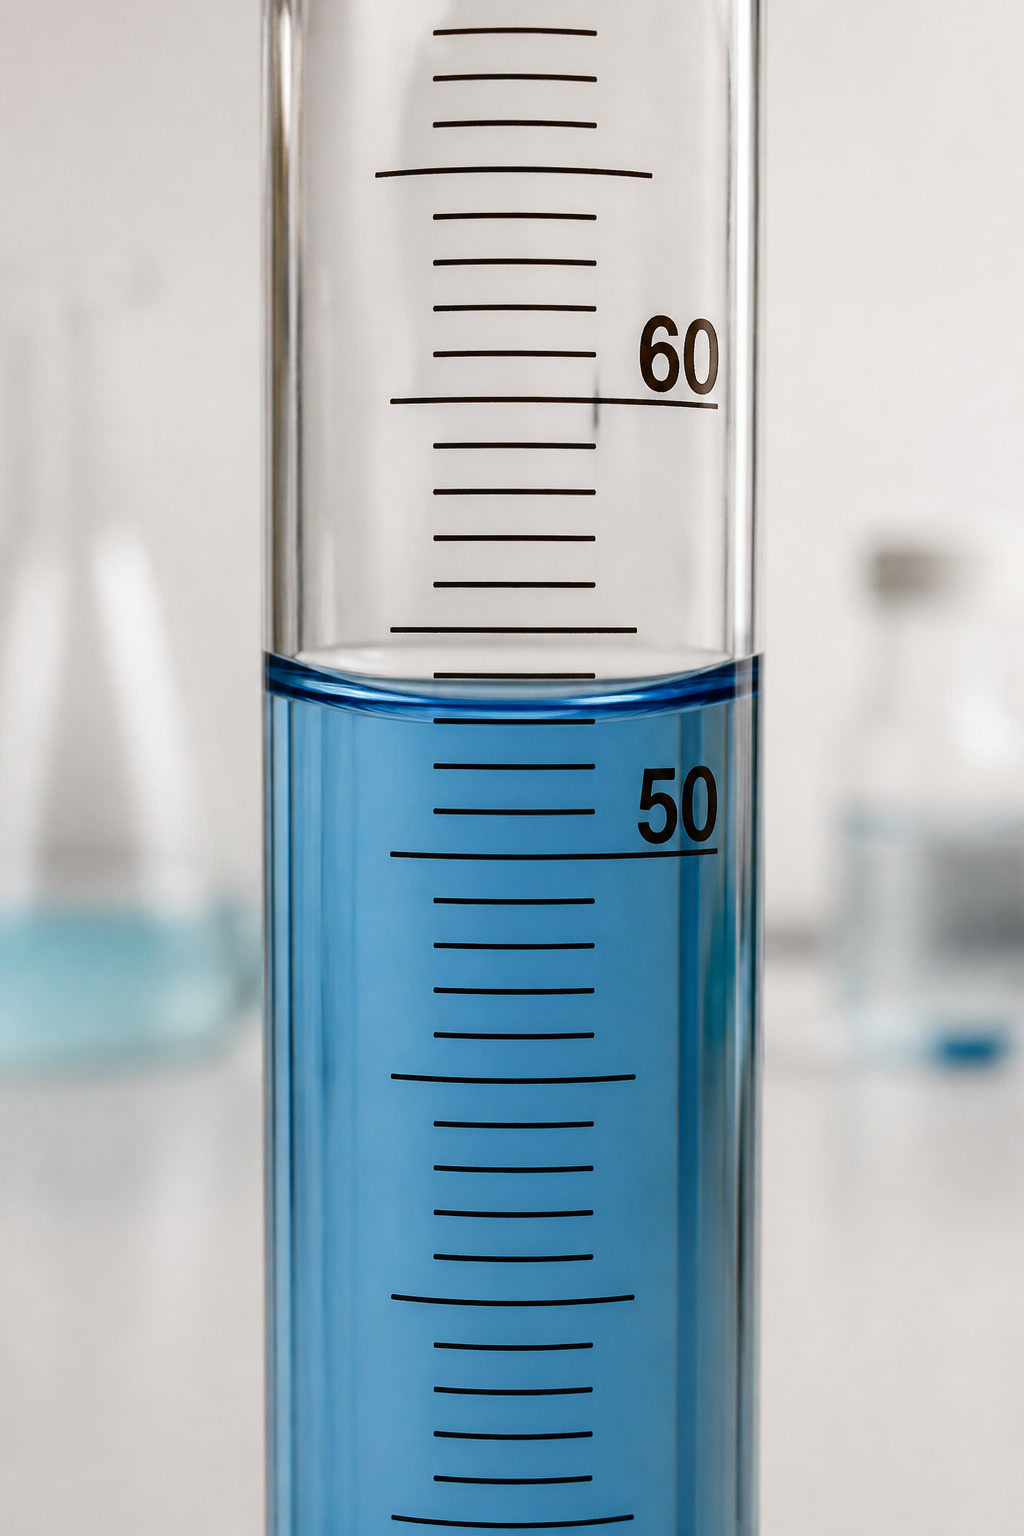
\includegraphics[width=0.3\linewidth]{images/book1/ai/g6-volume-cylinder.jpg}

{\small 弯月面特写：读取曲线中间平坦的部分，视线与该处齐平。}
\end{omfigure}

\section{测量固体 --- 即使是不规则的}

砖形固体可用尺子量出：长乘宽
再乘高，即得其体积 \unit{cm^3}，这在数学课上已学过。但石子、钥匙、李子呢？
尺子无法量取这种块状物。这个答案
已有两千年的历史，它出自一只
浴缸。

\begin{proposition}[排水]\label{prop:g6:mass-and-volume:displacement}
完全浸入水中的固体会排开——
与自身体积恰好相等的水。水面上升的高度
可以测量这个“闯入者”：无论是光滑还是
凹凸不平，水都会贴合它的每一处凹陷与凸起。
\end{proposition}

\begin{method}[用水面上升测体积]\label{met:g6:mass-and-volume:rise}
\begin{enumerate}
  \item 向量筒中注水，水量须足以盖住
        物体，并读出体积：例如 \qty{120}{mL}；
  \item 用细线系住物体，缓慢放入水中，
        使其完全浸没，不溅水，也不碰到量筒壁；
  \item 再读一次数，例如 \qty{145}{mL}；
  \item 作差：$145 - 120 = 25$——物体的体积为
        \qty{25}{cm^3}（上升水量以毫升计，
        石块以立方厘米计，两者数值相同）。
\end{enumerate}
\end{method}

\begin{omfigure}
\begin{tikzpicture}[scale=0.85]
  \draw[thick] (0.8,0) -- (0.8,3.6) (2.6,0) -- (2.6,3.6)
    (0.8,0) -- (2.6,0);
  \fill[omDef, opacity=0.2] (0.8,0.05) rectangle (2.6,2.0);
  \draw[omDef, very thick] (0.8,2.0) -- (2.6,2.0);
  \node[right, font=\footnotesize] at (2.7,2.0) {120};
  \node[below, font=\small] at (1.7,-0.3) {放入前};
  \draw[thick] (6.2,0) -- (6.2,3.6) (8.0,0) -- (8.0,3.6)
    (6.2,0) -- (8.0,0);
  \fill[omDef, opacity=0.2] (6.2,0.05) rectangle (8.0,2.42);
  \draw[omDef, very thick] (6.2,2.42) -- (8.0,2.42);
  \node[right, font=\footnotesize] at (8.1,2.42) {145};
  \draw (7.1,3.6) -- (7.1,1.0);
  \fill[omExo] (7.1,0.75) ellipse (0.4 and 0.3);
  \node[below, font=\small] at (7.1,-0.3)
    {放入后：石块完全没入水中};
  \draw[-Stealth, omThm, thick] (4.0,2.0) -- (5.6,2.35);
  \node[below, font=\small, omThm] at (4.8,1.9)
    {上升：\qty{25}{mL}};
\end{tikzpicture}

{\small 上升法：水面升高的体积恰好是
石块的体积——$145 - 120 = \qty{25}{cm^3}$。}
\end{omfigure}

\begin{example}[浴缸中的王冠]\label{ex:g6:mass-and-volume:archimedes}
相传国王怀疑金匠用白银掺假，偷换了王冠里的黄金，
便请科学家阿基米德在不损坏王冠的前提下，
查明真相。他踏进盛满水的浴缸，
看着水从盆沿溢出，他
突然醒悟：溢出的水量正是自身的体积，连凹凸之处也一并计入。
传说他跑遍街头，高呼“尤里卡！”
——\emph{我找到了！}至于王冠的体积如何揭穿骗局，
还需要再一个想法，将在两章之后讲解；浴缸让他
得到了测定\emph{任何}物体体积的办法。
\end{example}

\section{质量与体积是两个不同的答案}

\begin{example}[体积相同，质量不同]\label{ex:g6:mass-and-volume:different}
取两只相同的 \qty{25}{cL} 玻璃杯，一只装水，一只装蜂蜜，
称出它们的质量（减去杯子的质量）：装蜂蜜的那只
明显多出若干克，二者体积相同，
质量却不同。一升空气的质量只比一克多一点，
而同样一升水则重整整一千克。房间与物质
确实是两本不同的“账本”，请牢记这一点：
它将在本学年的最后一章中成为一条
有名字的定律。
\end{example}

\begin{remark}[如何单独称出容器中的物料]\label{rem:g6:mass-and-volume:tare}
怎样称面粉而不把碗一起称？现代天平通常带有
一个专门的按键：把空碗放在秤盘上，按下按键——
显示归零——然后倒入面粉：天平此时显示的
就只是面粉的质量。这一操作称为\emph{去皮}。没有此按键时，
可以称两次再相减：装有面粉的碗的质量减去空碗的质量。
两种方法遵循的仍是同一原则：
从一个可靠的零点出发。
\end{remark}

\section{练习}

\begin{exercise}[$\star$]\label{exo:g6:mass-and-volume:1}
体积回答的是什么问题，质量回答的
又是什么问题？请分别写出两者各自的两个主要单位。
\end{exercise}

\begin{exercise}[$\star$]\label{exo:g6:mass-and-volume:2}
换算下列各量：\qty{2}{L} 化为 \unit{cm^3}；\ \qty{350}{mL} 化为
\unit{cm^3}；\ \qty{1500}{cm^3} 化为升；\ 半升化为
毫升。
\end{exercise}

\begin{exercise}[$\star$]\label{exo:g6:mass-and-volume:3}
为什么读量筒时，必须把量筒放在桌面上，
视线与液面齐平，并读取弯月面的底部？请指出每条规则
分别防止了什么错误。
\end{exercise}

\begin{exercise}[$\star$]\label{exo:g6:mass-and-volume:4}
量筒读数为 \qty{200}{mL}；放入一颗李子后，读数为
\qty{265}{mL}。李子的体积为多少（以 \unit{cm^3} 计）？
\end{exercise}

\begin{exercise}[$\star$]\label{exo:g6:mass-and-volume:5}
为什么排水法对形状不规则的小石子也适用，即使
尺子根本无法测量它？哪条命题给出了解答？
\end{exercise}

\begin{exercise}[$\star$]\label{exo:g6:mass-and-volume:6}
一块砖形橡皮，长、宽、高分别为 \qty{5}{cm}、\qty{2}{cm}、
\qty{1}{cm}。它的体积是多少？验证方案：
若用排水法，你将如何验证这一结果？
\end{exercise}

\begin{exercise}[$\star$]\label{exo:g6:mass-and-volume:7}
称量大米：空碗质量为 \qty{280}{g}；装有大米的碗
质量为 \qty{745}{g}。大米的质量是多少？哪个按钮能
一步完成同样的工作？
\end{exercise}

\begin{exercise}[$\star$]\label{exo:g6:mass-and-volume:8}
体积更大的是一千克羽毛，还是一千克
铁？质量更大的是哪一个？（两个问题都请仔细作答。）
\end{exercise}

\begin{exercise}[$\star\star$]\label{exo:g6:mass-and-volume:9}
软木塞会漂浮，排水法对它失效。请提出一种改进方法，
仍使用量筒，并说明若改进方法用到辅助物体，
需要从读数中减去什么。
\end{exercise}

\begin{exercise}[$\star\star$]\label{exo:g6:mass-and-volume:10}
一盒果汁标注 \qty{1}{L}。倒出后，它可装满一个
\qty{250}{mL} 的杯子三次，第四杯只倒到
\qty{200}{mL} 刻度。这一标注是否属实？相差多少？
\end{exercise}

\begin{exercise}[$\star\star$]\label{exo:g6:mass-and-volume:11}
将一条项链放入读数为 \qty{80.0}{mL} 的量筒，它使
液面升至 \qty{83.5}{mL}。珠宝商称项链含有
\qty{5}{cm^3} 的黄金，这一说法可能成立吗？究竟是
什么被水测量出来了？
\end{exercise}

\begin{exercise}[$\star\star\star$]\label{exo:g6:mass-and-volume:12}
设计一种仿照浴缸的检验方法，用于检验
\cref{prop:g6:mass-and-volume:displacement} 本身，
用一个长方体形、尺子已可测出其体积的物体。写出
步骤，并预测两次量筒读数：将一块
$4 \times 3 \times 2$ 厘米的木块放入
\qty{150}{mL} 的水中，并说明何种结果能证明该命题
有误。
\end{exercise}

\section{周末问题：果园装瓶日}

\begin{problem}[{周末问题 --- 果园压榨日；
升数装瓶，箱子过秤；
壶中的小石子}]\label{pb:g6:mass-and-volume:1}
果园今天压榨苹果，每位帮手都有一项
测量任务。

\medskip\noindent\textbf{Part I --- 按升计的果汁。}
压榨机已装满一个 \qty{20}{L} 的桶。
\begin{enumerate}
  \item \qty{20}{L} 合多少立方厘米？
  \item 果汁装入 \qty{75}{cL} 的瓶中。这个桶可装满
        多少个\emph{整}瓶？
  \item 装完最后一个整瓶后，剩余果汁有多少，
        以厘升计？
  \item 将剩余果汁倒入 \qty{25}{cL} 的杯中。
        可以装满多少杯？
\end{enumerate}

\medskip\noindent\textbf{Part II --- 箱子过秤。}
\begin{enumerate}[resume]
  \item 一个空瓶质量为 \qty{450}{g}。利用第一部分，
        若每升果汁质量约为 \qty{1}{kg}，则一整瓶果汁的质量为多少？
        （请以克为单位计算。）
  \item 那么，一整瓶（包括空瓶）的质量共是多少？
  \item 一个木箱空箱重 \qty{2}{kg}，可装六
        整瓶。装满后的木箱总质量是多少？
  \item 货车最多可载 \qty{200}{kg} 的木箱。满载的木箱
        最多可装几箱？（只计整箱。）
\end{enumerate}

\medskip\noindent\textbf{Part III --- 壶中的小石子。}
小汤姆把一颗小石子放入装满 \qty{1}{L} 果汁的壶中，
果汁溢到了桌上。
\begin{enumerate}[resume]
  \item 擦干的溢出果汁量为 \qty{40}{mL}。它说明了小石子的
        什么量？依据哪条命题？
  \item 将小石子捞出后，壶中还剩
        多少果汁？
  \item 汤姆抗议：“小石子很小——你看，它能藏在
        我的拳头里！”他姐姐用量筒作答：
        她把小石子放入 \qty{100}{mL} 的水中，
        哪个读数能证明溢出量确实可信？
  \item 附加计算：小石子在厨房秤上的
        读数为 \qty{104}{g}。在不引入新概念的前提下，能否判断
        小石子的物质是比果汁的物质更重还是更轻，
        \emph{在占据相同体积时}？请比较
        \qty{40}{cm^3} 的小石子质量为 \qty{104}{g}，与
        充满同样 \qty{40}{cm^3} 的果汁，质量为多少？——
        请将你的结论留给密度一章。
\end{enumerate}
\end{problem}
